\documentclass[letterpaper, 12pt]{article}
\usepackage{pgfplots}
\usepgfplotslibrary{fillbetween}
\pgfplotsset{compat=1.13}

\title{Basics of Economics}
\author{Alvin Lin}
\date{Principles of Microeconomics: August 2016 - December 2016}

\begin{document}

\maketitle

\section{Model of an Economy}

\subsection{Production}
\textbf{The Economic Problem}: How are production decisions made?

\subsubsection{Production Possibilities Frontier (PPF)}
Determines the set of possible goods that can be produced at a given point in
time. It is the boundary between the combinations of goods that can be produced
and those that cannot be produced. The shape of the PPF curve is determined by
the resources available and the set of techniques available for producing
something. If you have a finite amount of a resource, your PPF will be
downwards sloping (true in almost all cases). Generally, the PPF is downwards
sloping and convex.

\subsubsection{Opportunity Cost (OC)}
The opportunity cost of an action is the highest valued alternative for
the action.

\paragraph{Example:} If I value fruits in the following pattern:
\[ mango > orange > apple \]
\begin{itemize}
  \item My OC is mango if I choose apple.
  \item My OC is mango if I choose orange.
  \item My OC is orange if I choose mango.
\end{itemize}

\paragraph{Example:} Two goods: grade on an economics exam (X), hours on a
video game (Y), 6 hours available in total. The total cost of each hour spent
on the game is:
\begin{center}
  \begin{tabular}{|c|c|}
    \hline
    hours played & points lost \\ \hline
    0 & 0 \\ \hline
    1 & 2 \\ \hline
    2 & 15 \\ \hline
    3 & 30 \\ \hline
    4 & 50 \\ \hline
    5 & 75 \\ \hline
    6 & 100 \\ \hline
  \end{tabular}
\end{center}

The marginal cost of each hour is:
\begin{center}
  \begin{tabular}{|c|c|}
    \hline
    hours played & marginal cost \\ \hline
    1 & 2 \\ \hline
    2 & 13 \\ \hline
    3 & 15 \\ \hline
    4 & 20 \\ \hline
    5 & 25 \\ \hline
    6 & 25 \\ \hline
  \end{tabular}
\end{center}

The PPF is:
\begin{center}
  \begin{tabular}{|c|c|}
    \hline
    hours played & test grade \\ \hline
    0 & 100 \\ \hline
    1 & 98 \\ \hline
    2 & 85 \\ \hline
    3 & 70 \\ \hline
    4 & 50 \\ \hline
    5 & 25 \\ \hline
    6 & 0 \\ \hline
  \end{tabular}
\end{center}

\subsection{Decreasing Marginal Benefit}
The more of a good we have, the less we are willing to give up for one more
unit. The total benefit is always increasing, while the marginal benefit always
decreases (but is always greater than 0). If we are maximizing our benefit,
we need to find the allocation efficiency (total benefit - total cost).
\begin{center}
  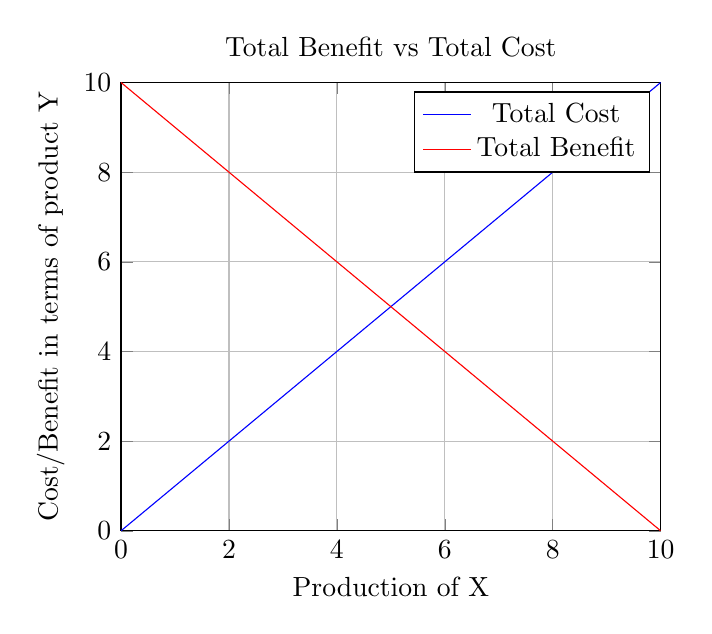
\begin{tikzpicture}
    \begin{axis} [
      title={Total Benefit vs Total Cost},
      xlabel={Production of X},
      ylabel={Cost/Benefit in terms of product Y},
      xmin=0, xmax=10,
      ymin=0, ymax=10,
      grid=both
    ]
    \addplot[color=blue] coordinates {(0,0) (10,10)};
    \addlegendentry{Total Cost};
    \addplot[color=red] coordinates {(0,10) (10,0)};
    \addlegendentry{Total Benefit};
    \end{axis}
  \end{tikzpicture}
\end{center}
The allocation efficiency is maximized where the total cost and total benefit
meet.

\subsubsection{Practice Problem 1}
\begin{center}
  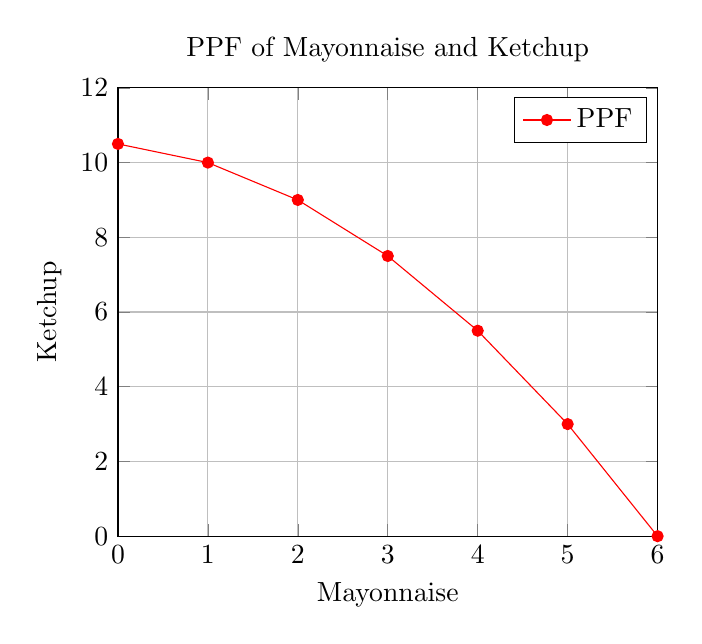
\begin{tikzpicture}
    \begin{axis} [
      title={PPF of Mayonnaise and Ketchup},
      xlabel={Mayonnaise},
      ylabel={Ketchup},
      xmin=0, xmax=6,
      ymin=0, ymax=12,
      grid=both
    ]
    \addplot[color=red, mark=*] coordinates {
      (0,10.5)(1,10)(2,9)(3,7.5)(4,5.5)(5,3)(6,0)
    };
    \addlegendentry{PPF}
    \end{axis}
  \end{tikzpicture}
  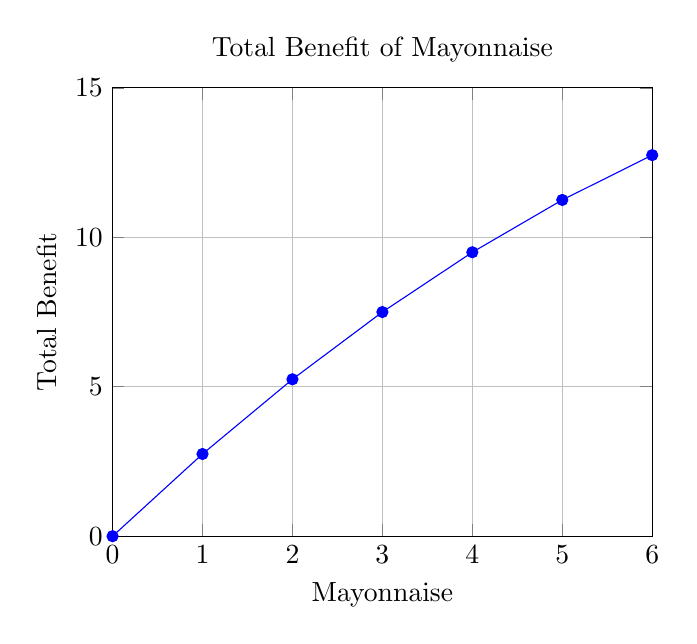
\begin{tikzpicture}
    \begin{axis} [
      title={Total Benefit of Mayonnaise},
      xlabel={Mayonnaise},
      ylabel={Total Benefit},
      xmin=0, xmax=6,
      ymin=0, ymax=15,
      grid=both
    ]
    \addplot[color=blue, mark=*] coordinates {
      (0,0)(1,2.75)(2,5.25)(3,7.5)(4,9.5)(5,11.25)(6,12.75)
    };
    \end{axis}
  \end{tikzpicture}
\end{center}
What is the allocative efficient amounts of \( x_{1} \) and \( y \)?
\[ \mathrm{Allocative\ efficiency} = MC - MB \]
\begin{center}
  \begin{tabular}{|c|c|c|}
    \hline
    x & marginal cost & marginal benefit \\ \hline
    1 & 0.5  & 2.75 \\ \hline
    2 & 1    & 2.5  \\ \hline
    3 & 1.5  & 2.25 \\ \hline
    4 & 2    & 2    \\ \hline
    5 & 2.5  & 1.75 \\ \hline
    6 & 3    & 1.5  \\ \hline
  \end{tabular}
\end{center}
Producing 4 units of mayonnaise and 5.5 units of ketchup will maximize
production as well as benefit.

\subsubsection{Practice Problem 2}
Suppose you wake up one morning and discover that mayonnaise is good for your
health. What happens to allocative efficiency?
\begin{center}
  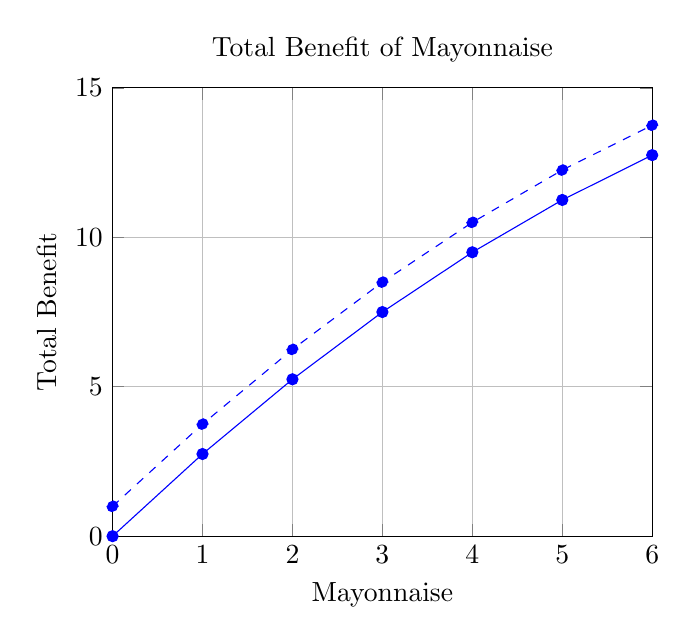
\begin{tikzpicture}
    \begin{axis} [
      title={Total Benefit of Mayonnaise},
      xlabel={Mayonnaise},
      ylabel={Total Benefit},
      xmin=0, xmax=6,
      ymin=0, ymax=15,
      grid=both
    ]
      \addplot[color=blue, mark=*] coordinates {
        (0,0)(1,2.75)(2,5.25)(3,7.5)(4,9.5)(5,11.25)(6,12.75)
      };
      \addplot[color=blue, mark=*, dashed] coordinates {
        (0,1)(1,3.75)(2,6.25)(3,8.5)(4,10.5)(5,12.25)(6,13.75)
      };
    \end{axis}
  \end{tikzpicture}
\end{center}
The marginal benefit curve of mayonnaise will shift upwards, causing us to
consume more mayonnaise and less ketchup.

\subsubsection{Practice Problem 3}
Suppose it is a great season for your tomato garden. There are more resources
available to produce ketchup with. What happens to the marginal cost and
benefit of ketchup and mayonnaise?
\begin{center}
  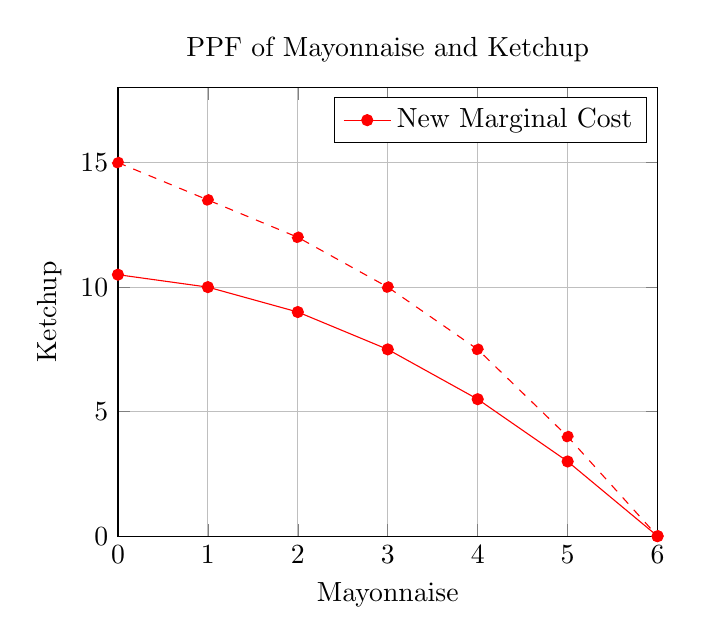
\begin{tikzpicture}
    \begin{axis} [
      title={PPF of Mayonnaise and Ketchup},
      xlabel={Mayonnaise},
      ylabel={Ketchup},
      xmin=0, xmax=6,
      ymin=0, ymax=18,
      grid=both
    ]
    \addplot[color=red, mark=*] coordinates {
      (0,10.5)(1,10)(2,9)(3,7.5)(4,5.5)(5,3)(6,0)
    };
    \addplot[color=red, mark=*, dashed] coordinates {
      (0,15)(1,13.5)(2,12)(3,10)(4,7.5)(5,4)(6,0)
    };
    \addlegendentry{New Marginal Cost}
    \end{axis}
  \end{tikzpicture}
  \noindent\rule{13.7cm}{0.4pt}
  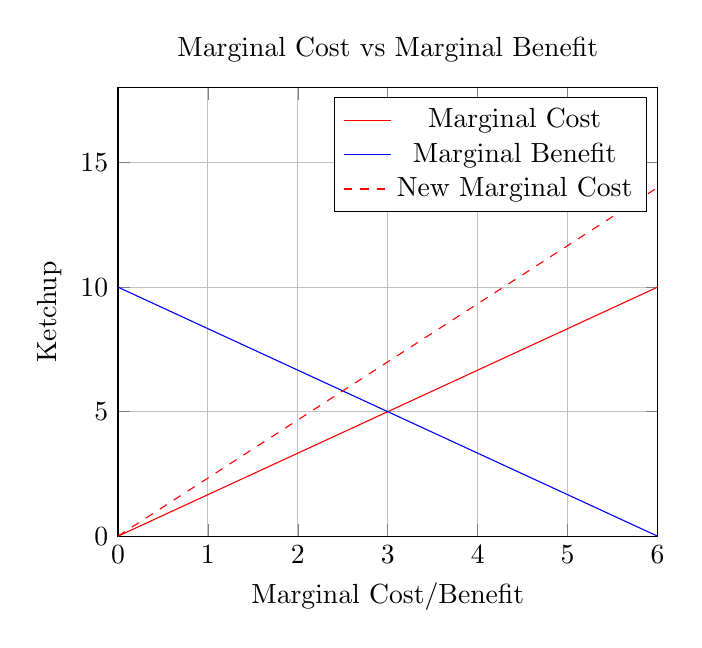
\begin{tikzpicture}
    \begin{axis} [
      title={Marginal Cost vs Marginal Benefit},
      xlabel={Marginal Cost/Benefit},
      ylabel={Ketchup},
      xmin=0, xmax=6,
      ymin=0, ymax=18,
      grid=both
    ]
    \addplot[color=red] coordinates {
      (0,0)(6,10)
    };
    \addlegendentry{Marginal Cost}
    \addplot[color=blue] coordinates {
      (0,10)(6,0)
    };
    \addlegendentry{Marginal Benefit}
    \addplot[color=red, dashed] coordinates {
      (0,0)(6,14)
    };
    \addlegendentry{New Marginal Cost}
    \end{axis}
  \end{tikzpicture}
\end{center}
The marginal cost for ketchup will increase since you are able to produce more.
For each unit of mayonnaise you produce, you give up more ketchup that could
have been produced.

\subsection{Gains From Trade}
People could produce all the goods they consume on their own, or they could
specialize and conduct trade.
\newline
\textbf{Comparative Advantage (CA)}: A person (or country) has a comparative
advantage in an activity if they can perform that activity at a lower
opportunity cost that everyone else.
\newline
\textbf{Absolute Advantage (AA)}: A person (or country) has an absolute
advantage if they are more productive than others.
\begin{center}
  \begin{tabular}{|c|c|c|}
    \hline
    \multicolumn{3}{|c|}{Example 1} \\ \hline
           & Autos & Natural Gas  \\ \hline
    US     & 300 & 100            \\ \hline
    Canada & 60  & 80             \\ \hline
  \end{tabular}
\end{center}
In this example, the opportunity cost for Canada is \( \frac{3}{4} \) autos in
terms of natural gas, while the opportunity cost for the US is 3
autos in terms of natural gas. Therefore, Canada has a comparative advantage
in natural gas. Conversely, if this is the case, the the US must have a
comparative advantage in autos. \par
However, the US has an \textbf{absolute advantage} in natural gas and autos
since they produce more. \par
Whenever a country has a comparative advantage, it is always possible to
realize gains from trade.
\begin{center}
  \begin{tabular}{|c|c|c|}
    \hline
    \multicolumn{3}{|c|}{Example 2} \\ \hline
           & Autos & Natural Gas  \\ \hline
    US     & 150 & 50             \\ \hline
    Canada & 30  & 40             \\ \hline
    Totals & 180 & 90             \\ \hline
  \end{tabular}
\end{center}
If Canada were to shift more production to natural gas and the US were to shift
production to autos, then there would be a greater total of both.
\begin{center}
  \begin{tabular}{|c|c|c|}
    \hline
    \multicolumn{3}{|c|}{After Specializing} \\ \hline
           & Autos & Natural Gas  \\ \hline
    US     & 240 & 20             \\ \hline
    Canada & 0   & 80             \\ \hline
    Totals & 240 & 100            \\ \hline
  \end{tabular}
\end{center}

\begin{center}
  If any errors are found, please contact me at alvin.lin.dev@gmail.com
\end{center}

\end{document}
